\documentclass[9pt,twocolumn,twoside]{osajnl}
%% Please use 11pt if submitting to AOP
% \documentclass[11pt,twocolumn,twoside]{osajnl}

\journal{ol} % Choose journal (ao, aop, josaa, josab, ol)

% See template introduction for guidance on setting shortarticle option
\setboolean{shortarticle}{true}
% true = letter / tutorial
% false = research / review article
% (depending on journal).

\title{Distribution of twin beam at 1550 nm telecom band over 26 km optical fiber}

\author[1]{Yuhong Liu, Nan Huo}
\author[1,*]{Xiaoying Li}


\affil[1]{College of Precision Instrument and Opto-electronics Engineering, Tianjin University, Key Laboratory of Optoelectronics Information Technology of Ministry of Education, Tianjin 300072, China}

\affil[*]{Corresponding author: xiaoyingli@tju.edu.cn}

%% To be edited by editor
% \dates{Compiled \today}

\ociscodes{(270.0270) Quantum Optics; (060.4370) Nonlinear optics, fibers; (190.4380) Nonlinear optics, four wave mixing}

%% To be edited by editor
% \doi{\url{http://dx.doi.org/10.1364/XX.XX.XXXXXX}}

\begin{abstract}
We experimentally measured 5.8dB intensity squeezing generated by all-fiber system and demonstrated transmission of intensity squeezing state in 26 km telecom single mode fiber while maintaining 2dB squeezing.
Our experiment shows that the long-haul transmission of intensity squeezed state does not introduce additional noise to the intensity squeezed state.
% Our result shows that the primary limit of measured squeezing is the loss of transmission fiber, which can be improved by low loss fibers.
\end{abstract}

\setboolean{displaycopyright}{true}

\begin{document}

\maketitle
%%%%%%%%%%%% Introduction %%%%%%%%%%%%%%%%%%%%%%%%%%%%%%%%%%%%%%%%%%%%%
\section{Introduction}


Creation and distribution of the continuous-variable quantum states are important for quantum communication applications, such as teleportation, dense coding and quantum key distribution\cite{braunstein_quantum_2005}.
For long distance quantum communication protocols, such as quantum key distribution and quantum teleportation, transmitting quantum state far enough while keeping its quantum property is essential.
Modern fiber communication networks are able to transmit light in telecom band with little loss, which is very promising for quantum communication.
There has been much endeavor in trying to transmit quantum states further[Satellite, Fiber, Air] and transmit quantum state with low loss fiber network is a nice solution.
We present an all-fiber pulsed twin beams source in telecom band which is compatible with fiber telecommunication networks.
The intensity difference squeezing out of our source is distributed over 26km single mode fiber (SMF) and still remain 2dB squeezing, which is the longest for continuous variable state distribution.
%The directly measured intensity difference squeezing is $R_{0}= 5.8$ dB.%, which is the best reported in fiber system.
%Besides, twin beams generated in telecom band by fiber system are compatible with conventional single mode fiber (SMF). %, and suffers way much less coupling loss into SMF. % (around 4\% splicing loss and can be less if the fibers are properly tapered before splicing) than those generated by crystals and atom systems.%degrades the squeezing by introducing new vacuum.
%The twin beams are transmitted by individual SMFs for long distance to test its vulnerability to transmission loss and other noise.
%After distribution in SMF for 4, 10, 16 and 26km, the measured normalized noise power is still 2dB below shot noise limit defined by detected intensity.
Comparing the experimental results with the theoretically expected values, we find that the only limitation for further propagation is the fiber transmission loss. Pulsed nature of our twin beams source provide further advantages over continuous wave squeezing which suffers from stimulated Brillouin scattering\cite{feng_distribution_2017}.
%, which can be improved with the help of low loss fiber.
%Thus, our twin beam source has great potential in quantum information and quantum cryptology.



Intensity squeezing is a useful tool for quantum information, quantum metrology and some other things that I don't know. In experiment that xxxxx, it's important to transmit quantum state far enough while keeping its quantum property.

XXXXXXX

% basic results
In this letter, we present a pulsed twin beam source in telecom band via Stimulated Four Wave Mixing (FWM) in Dispersion Shifted Fiber (DSF) and transmit it by two Single Mode Fiber (SMF). The initial directly measured intensity directly difference squeezing is $R_{0}= 6 dB$, which is the best reported in fiber system. Besides, twin beams generated in telecom band by fiber system are compatible with conventional SMF, and suffers less coupling loss, which is generally inevitable for those generated by crystals and atom systems.%degrades the squeezing by introducing new vacuum.

We managed to lunch the twin beams into individual SMF.
After propagating in SMF for 10km, the measured normalized noise power is still 2dB below shot noise limit defined by detected intensity. Comparing to theoretical prediction, the only limitation for further propagation is the fiber transmission loss, which can be improved with the help of low loss fiber. Thus, our twin beam source has great potential in quantum information and quantum cryptology.


\section{Setup}

\begin{figure}[htbp]
\centering
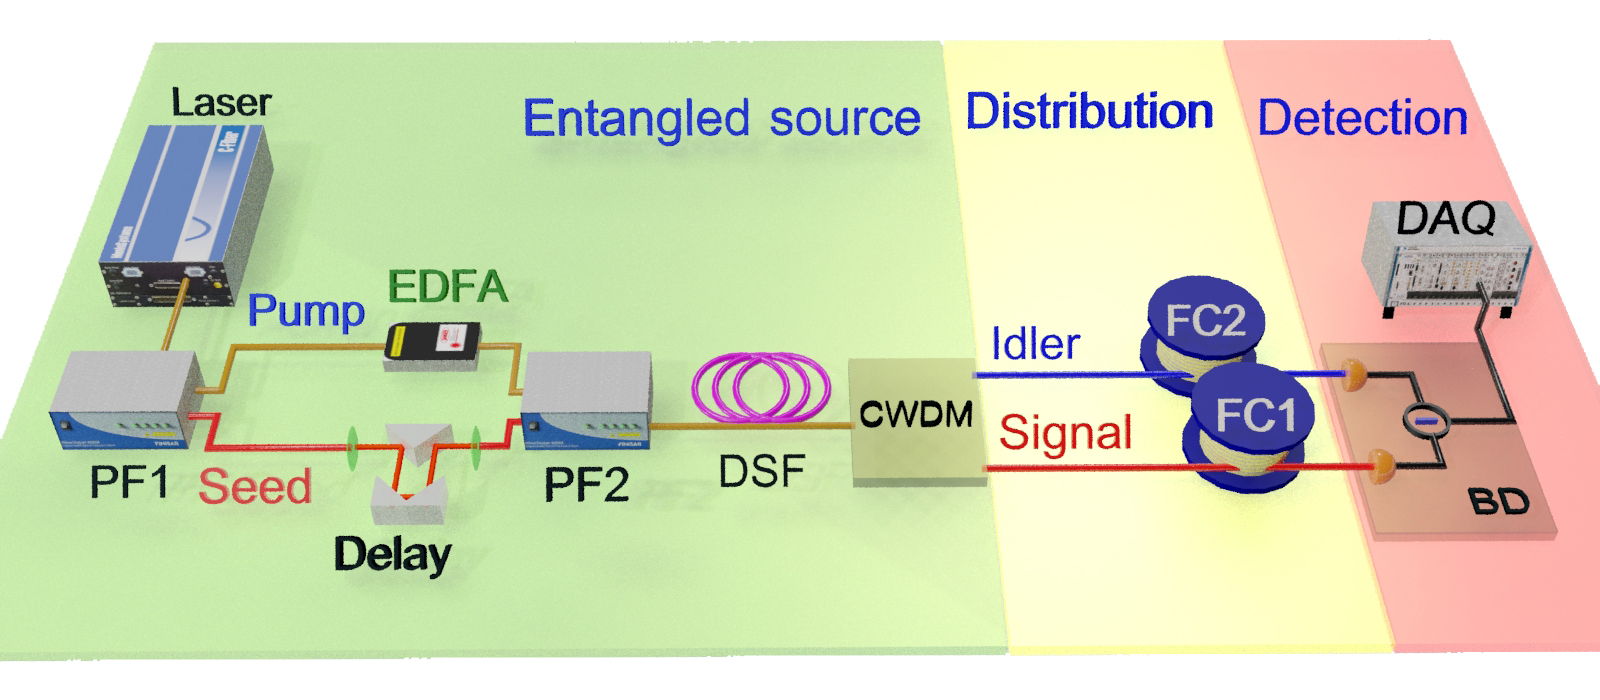
\includegraphics[width=\linewidth]{fig1_3d_2.jpg}
\caption{Experiment setup.
PF1-2, programmable optical filter;
EDFA, erbium-doped fiber amplifier;
Delay, mechanical delay line;
DSF, dispersion shifted fiber;
CWDM, coarse wavelength division multiplexers;
FC1-2, fiber coil;
BD, balanced detector;
DAQ, data acquisition system}
\label{fig_setup}

\end{figure}
The experiment setup is shown in Fig. \ref{fig_setup}.
The non-degenerate twin beams are generated from a pulse pumped fiber optical parametric amplifier (FOPA) utilizing four wave mixing effect between strong pump and week seed injection via \(\chi^{(3)} \) nonlinear interaction in 300 m DSF fiber.
The zero dispersion wavelength of DSF is 1548.5 nm when cooled at 77 k by liquid nitrogen, which reduces additional raman noise in generated twin beams \cite{guo12}.
The Zero Dispersion Wavelength (ZDW) of DSF is 1552.6 at room temperature and shifts to 1548.5 nm when cooled at 77k by liquid nitrogen, which improves the quality of generated twin beam \cite{guo12}.
%% filter
For simplicity of narration, we denote the beam in shorter injecting wavelength signal and the conjugate beam in longer wavelength as idler.
The pump and seed are filtered separately from a mode-locked laser by Programable Filter (PF1), and the center wavelength and bandwidth of pump (seed) are 1549.5 nm (1533 nm) and 0.7 nm (1.5 nm) respectively.
After PF1, the filtered pump is further amplified by Erbium-doped Fiber Amplifier (EDFA) to meet the required power while the seed is delayed by a mechanical delay-line so as to keep overlapped with pump in DSF.
The amplified pump and seed is combined at the PF2 and feed into DSF where twin beam generated via FWM.
Besides, PF2 also filter out ASE from EDFA and compensate dispersion from previous fiber system, which helps to increase the gain of OPA.
% Further more, PF2 can generate arbitrary dispersion on pump and injected signal, which helps optimize the mode match condition of FWM \cite{GuoOL16}.
%The DSF used as gain media is soaked in liquid nitrogen, which improves the quality of generated twin beam \cite{guo12}.

After amplification in DSF, twin beam is generated and separated by 15nm bandwidth Coarse Wavelength Division Multiplexer (CWDM), which has 90\% and 86\% transmission efficiency in signal (centered at 1531nm) and idler channel (centered at 1571nm)  respectively with DSF-SMF splicing loss at the output of DSF and SMF-SMF splicing loss between CWDM filters included.

The separated twin beam is transmitted individually by single mode Fiber Coil FC1 and FC2, which has equal length so as to simplify the detection system.
The SMF used has typical 0.2dB/km transmission loss and the length is set to 0, 2, 5, 8 and 13km, corresponding to distribution of entangled source by 0, 4, 10, 16, 26km respectively, so as to demonstrate the potential of twin beam in long haul quantum resource distribution.
The signal and idler of twin are detected by a Balanced Detector (BD) directly. The BD used in our experiment is modified Thorlabs PDB450C, whos detectors are replaced by high quantum efficiency (98\% with coupling efficiency included) InGaAs Pin detectors from Laser Components.
To balance the intensity difference between signal and idler field caused by stimulated Raman amplification, the idler field is attenuated slightly(1-2\%)\cite{guo12}.

%%%%%% CLEO
\section{CLEO}
The experiment setup is shown in Fig. \ref{fig_setup}.
The non-degenerate twin beams are generated from a pulse pumped fiber optical parametric amplifier (FOPA) utilizing four wave mixing effect between strong pump and week seed injection via \(\chi^{(3)} \) nonlinear interaction in 300 m DSF fiber.
The zero dispersion wavelength of DSF is 1548.5 nm when cooled at 77 k by liquid nitrogen, which reduces additional raman noise in generated twin beams \cite{guo12}.
The wavelengths of pump and injection signal  are 1549.5 nm and 1533 nm, at which the phase matching condition of FWM is satisfied in the DSF.
The filtered pump after F1 is further amplified by an erbium-doped fiber amplifier (EDFA) to meet the required power.
The seed is delayed by a mechanical delay-line so as to keep overlapped with pump in DSF.
The injection and pump are combined by a dual channel filter F2 and launched into the DSF.
At the output of DSF, the amplified signal and idler filed are separated from the residual pump by a coarse wavelength division multiplexers (CWDM).
We then propagate the signal and idler beam through SMF1 and SMF2 and measure the remaining intensity difference by using the balanced detector (BD) equipped with high quantum efficiency (96.5\% with coupling efficiency included) InGaAs detectors.
%%%%%%%%%%%%%%%%%%%%%%%%% transmission
The SMF in this experiment has 0.2 dB/km transmission loss and the length for distribution of twin beams is set to 0, 4, 10, 16 and 26 km, so as to demonstrate the potential of twin beams in long haul quantum resource distribution.
%The signal and idler of twin are detected directly by a balanced detector (BD) with high quantum efficiency (96.5\% with coupling efficiency included) InGaAs detectors.
%To balance the intensity difference between signal and idler field caused by stimulated Raman amplification, the idler field is attenuated slightly(1-2\%)\cite{guo12}.

%During FWM process, twin beam is generated by amplifying injected seed via \(\chi^{(3)} \) nonlinear interaction with strong pump.


%The amplified pump and seed is combined at the F2 and feed into DSF where twin beams are generated.
% Further more, PF2 can generate arbitrary dispersion on pump and injected signal, which helps optimize the mode match condition of FWM \cite{GuoOL16}.
%The DSF used as gain media is soaked in liquid nitrogen, which improves the quality of generated twin beam \cite{guo12}.
%For simplicity of narration, we denote the beam in shorter seed wavelength (1533 nm) as signal and the conjugate beam in longer wavelength (1566 nm) as idler.
%After amplification in DSF, twin beams are generated and separated by 15 nm bandwidth coarse wavelength division multiplexers (CWDM).% shown in Fig. \ref{fig_setup}, which has 92\% and 88\% transmission efficiency in signal (centered at 1531nm) and idler channel (centered at 1571nm) respectively with DSF-SMF splicing loss (3.6\%)at the output of DSF and SMF-SMF splicing loss($<1\%$) between CWDM filters included.


\section{Results}

We first measure the twin beam directly after the generation so as to evaluate the quality.
Intensity difference squeezing of twin beam is evaluated by the ratio between intensity difference noise of twin beam and SNL at identical intensity on detectors of BD.
Fig. \ref{fig2_OPA}(a) shows the measured intensity difference squeezing at different OPA gain with the insert showing the gain of OPA at different pump power.
It can be seen that the maximum squeezing reached in our experiment is 5.8dB when the power gain of OPA is arond 30.
The measured squeezing decrease slightly when the gain of OPA increase further, which is probably caused by raman effect who introduce additional noise to both signal and idler field.

In fig. \ref{fig2_OPA}(b) shows the best noise reduction result read on the DAQ system when pump power is 1.4 mW and intensity of signal and idler field is both around 15 uW. Line(2) is the intensity difference noised with line(1) is recorded corresponding SNL with identical intensity. It's obvious to around 5.8 dB noise reduction from SNL. Even though, the best result cancels out Electronic Noise (EN) shown by line3, the influence over uncorrected squeezing is no more than a slight change.

\begin{figure}[htbp]
\centering
\includegraphics[width=\linewidth]{Gain_and_sqz_vertical.jpg}%{Gain_and_sqz.jpg}
\caption{Performance of intensity difference squeezing. (a) Gain curve. (b) Maximum intensity difference squeezing measured. (c) SQZ vs Power gain}
\label{fig2_OPA}
\end{figure}

According to previous works [???], for twin beam possess $R_0$ initial intensity difference squeezing, the measurable intensity difference squeezing $ R(\eta)$ after detecting with quantum efficiency $\eta$ can be simplified as:
\begin{equation}
R(\eta) = 1+\eta(R_0-1)
\label{eq:loss}
\end{equation}

This relations defines the upper limit of quantum resource left after a certain amount of loss. According to this relation, the normalized intensity noise generated from OPA is more than 7dB after efficiency correction(90\% for signal field and 85 for idler field).	



Based on this equation, we calculated the normalized intensity noise at different transmission loss after CWDMs and plotted by blue line in fig. \ref{fig_loss}. The top axis is the signal field detection efficiency, and the bottom axis is the length of SMF that cause same amount of transmission loss. As shown in the figure, intensity squeezing can endure a pretty long SMF transmission and keep more than 2dB squeezing after distributing the twin beam by 26km, which means 13km SMF on signal and idler channel respectively.

\begin{figure}[htbp]
\centering
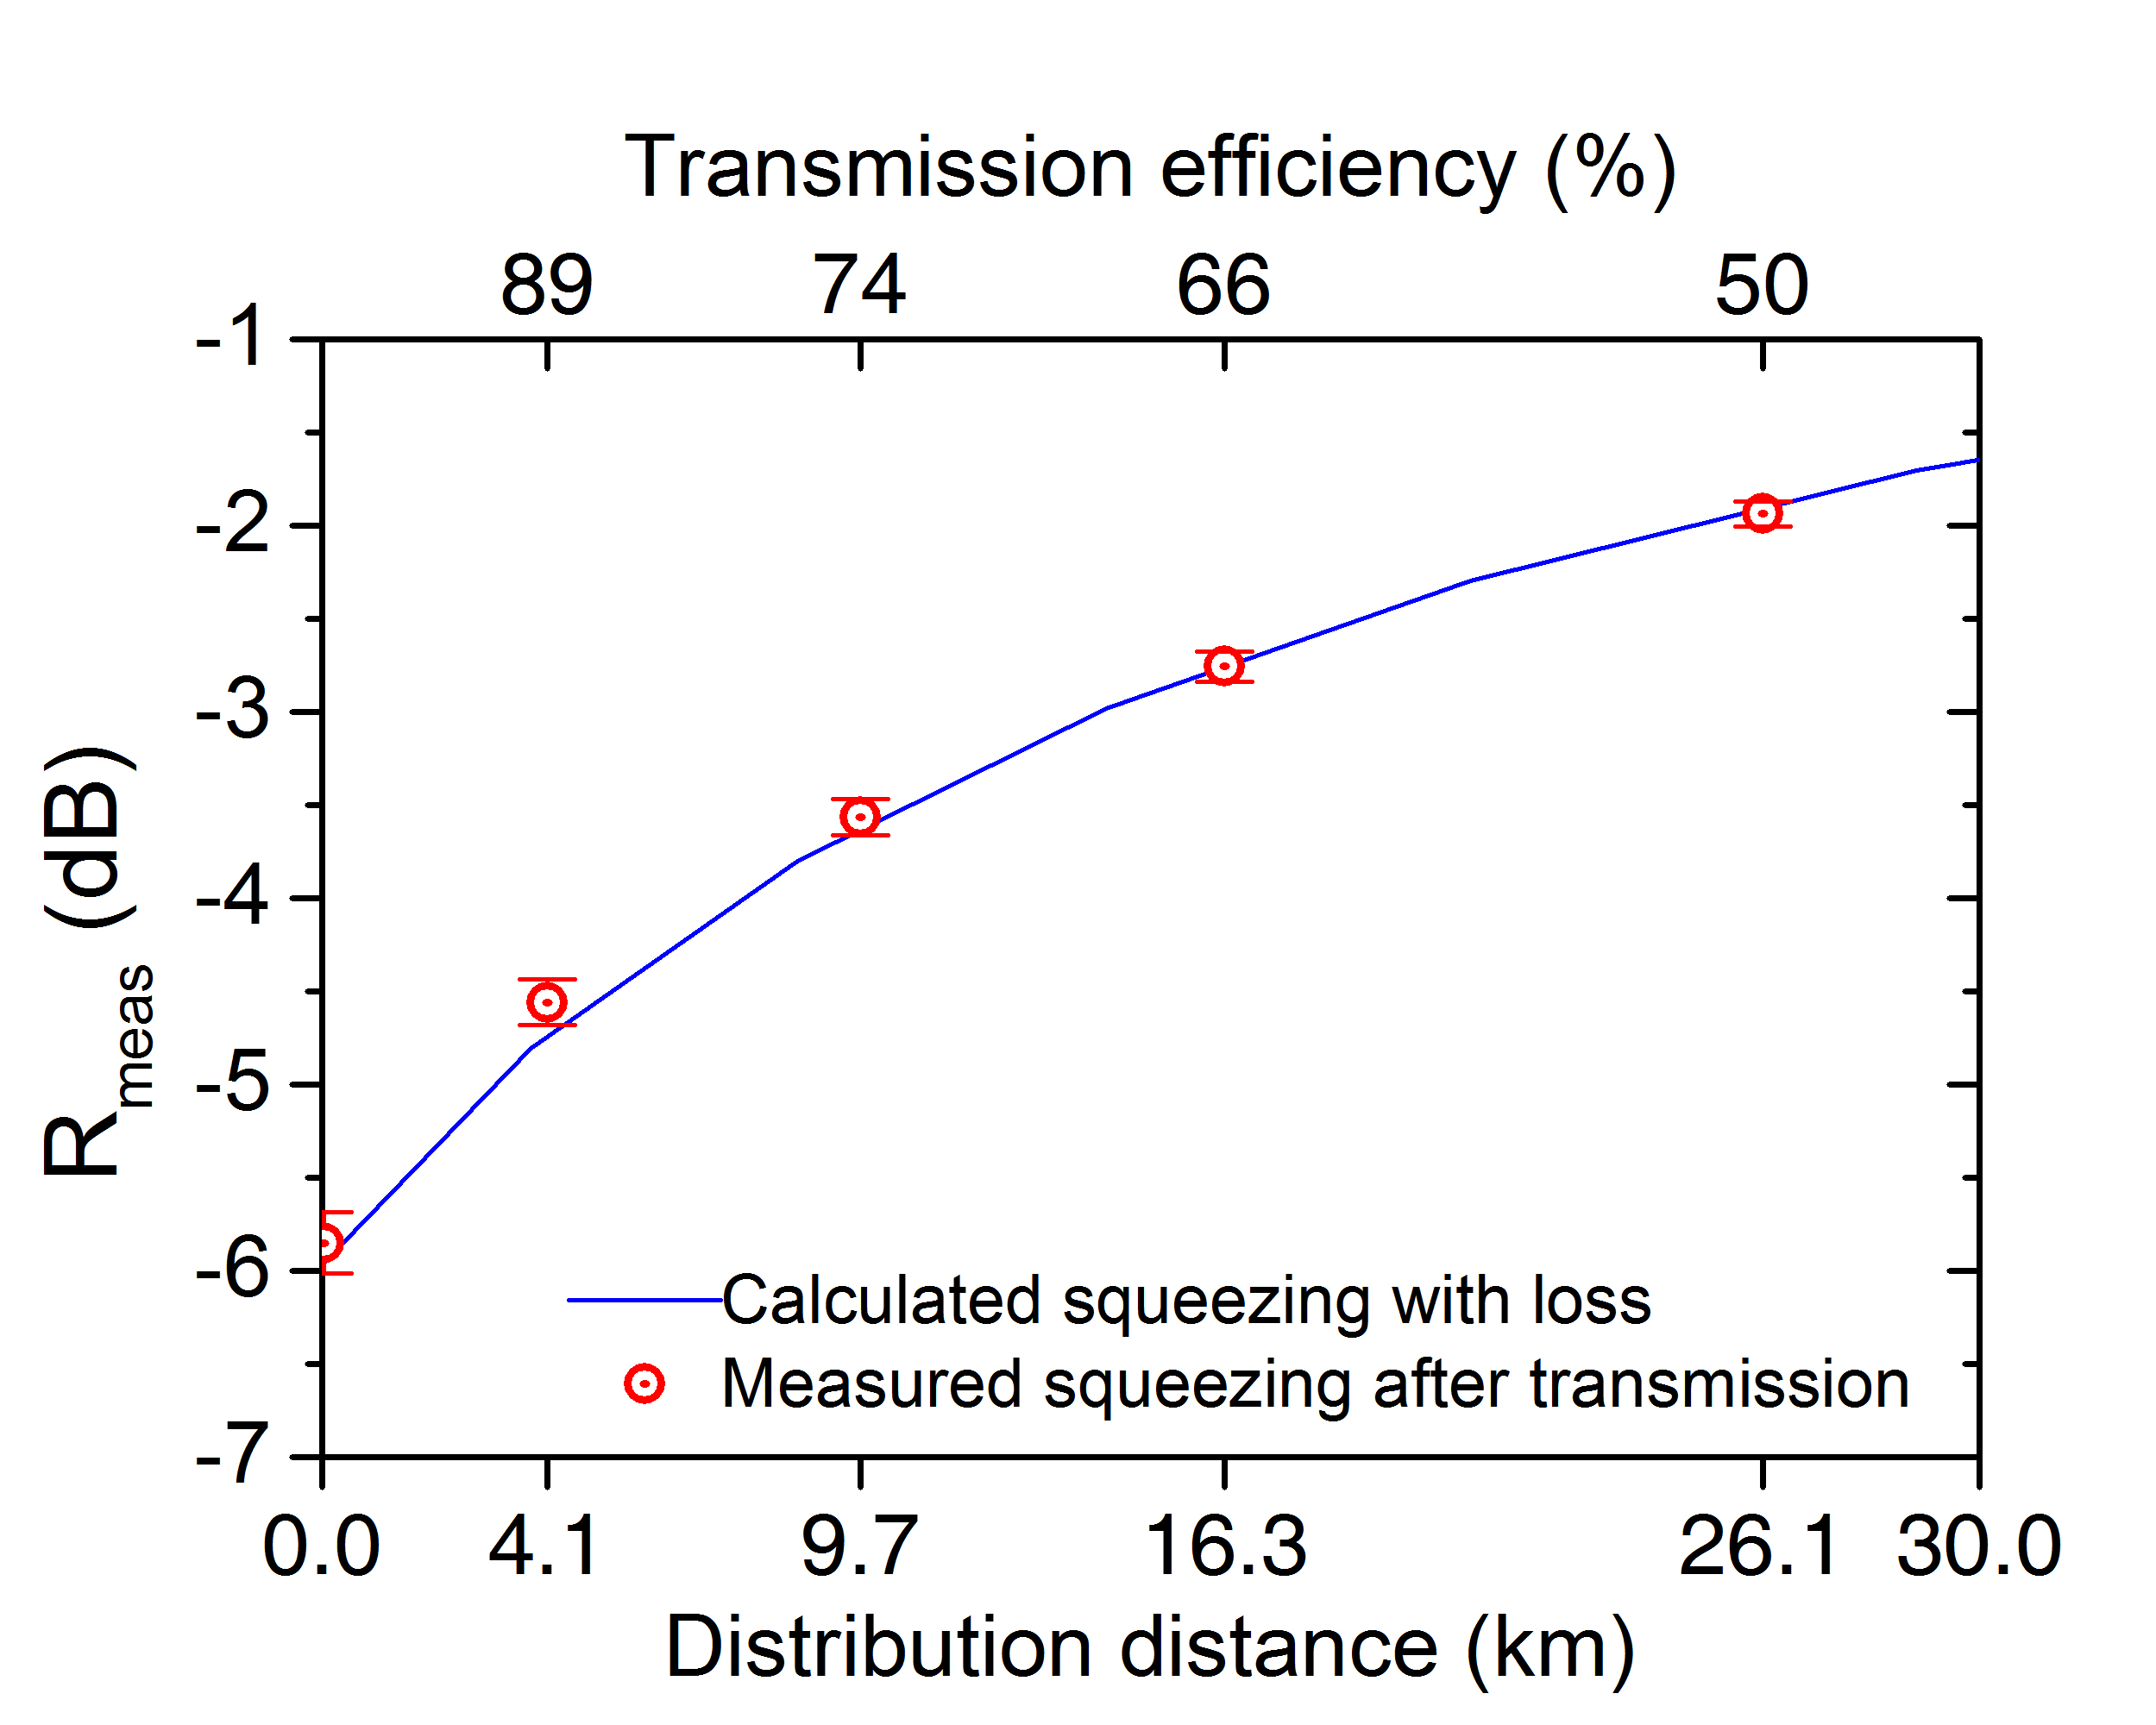
\includegraphics[width=\linewidth]{Sqz_vs_Length_dB_color.jpg}
\caption{Measurable intensity difference squeezing at different transmission loss}
\label{fig_loss}
\end{figure}

After analysis above, we lunch the generated twin beam into two SMF, the output from two SMF are detected by BD show in fig. \ref{fig_setup}.
After different length of fiber, the attenuation caused by fiber transmission loss makes the measured intensity squeezing degrade accordingly.
The relation between fiber length and measured normalized intensity difference noise is plot as red dots in fig. \ref{fig_loss}.
Comparing to theoretical prediction plot as blue line, the experiment result agrees well with the equation (\ref{eq:loss}), which means there is no other additional noise introduced while distributing the twin beam and the only limitation is the transmission loss of SMF, which can be improved by utilizing ultra low loss fibers that introduce 0.16 dB/km transmission loss [???find someone].


\section{Conclusion}
In conclusion, we experimentally built an all fiber twin beam source that possess 5.8 dB direct measurable intensity squeezing.
The generated twin beam is distributed by 26 km and still remains 2 db squeezing, which fits theoretical prediction well. Considering our all fiber twin beam source is the best in record (5.8dB) and pretty compatible with conventional fiber communication systems, this source shows great potential in quantum conmmucation and long distance quantum metrology.


\section{Funding Information}
Thanks for collaborators helping me with instrument coordination and Wei Zhang, Zhiqun Yang providing useful discussion and one of the Waveshaper. Thanks my wife for tolerating my endless typing in the mid night.

This work is supported by the XXXX.


\section{References}

Note that \emph{Optics Letters} uses an abbreviated reference style. Citations to journal articles should omit the article title and final page number; this abbreviated reference style is produced automatically when the \emph{Optics Letters} journal option is selected in the template, if you are using a .bib file for your references.

However, full references (to aid the editor and reviewers) must be included as well on a fifth informational page that will not count against page length; again this will be produced automatically if you are using a .bib file.

\bigskip
\noindent Add citations manually or use BibTeX. See \cite{Zhang:14,OSA,FORSTER2007,testthesis,guo12}.

% Bibliography
\bibliography{10km_sqeezing}

% Full bibliography added automatically for Optics Letters submissions; the following line will simply be ignored if submitting to other journals.
% Note that this extra page will not count against page length
\bibliographyfullrefs{10km_sqeezing}

%Manual citation list
%\begin{thebibliography}{1}
%\bibitem{Zhang:14}
%Y.~Zhang, S.~Qiao, L.~Sun, Q.~W. Shi, W.~Huang, %L.~Li, and Z.~Yang,
 % \enquote{Photoinduced active terahertz metamaterials with nanostructured
  %vanadium dioxide film deposited by sol-gel method,} Opt. Express \textbf{22},
  %11070--11078 (2014).
%\end{thebibliography}

% Please include bios and photos of all authors for aop articles
\ifthenelse{\equal{\journalref}{aop}}{%
\section*{Author Biographies}
\begingroup
\setlength\intextsep{0pt}
\begin{minipage}[t][6.3cm][t]{1.0\textwidth} % Adjust height [6.3cm] as required for separation of bio photos.
  \begin{wrapfigure}{L}{0.25\textwidth}
    
\includegraphics[width=0.25\textwidth]{john_smith.eps}
  \end{wrapfigure}
  \noindent
  {\bfseries John Smith} received his BSc (Mathematics) in 2000 from The University of Maryland. His research interests include lasers and optics.
\end{minipage}
\begin{minipage}{1.0\textwidth}
  \begin{wrapfigure}{L}{0.25\textwidth}
    
\includegraphics[width=0.25\textwidth]{alice_smith.eps}
  \end{wrapfigure}
  \noindent
  {\bfseries Alice Smith} also received her BSc (Mathematics) in 2000 from The University of Maryland. Her research interests also include lasers and optics.
\end{minipage}
\endgroup
}{}

\end{document}